\section{Parser}

\begin{frame}
	\frametitle{Parser - Allgemein}
	\begin{itemize}
		\item Verwendete Werkzeuge: Happy, Alex
		\item Input: Tokens
		\item Output: ABSTree
		\item Herausforderungen:
			\begin{itemize}
				\item Integration in Build System
				\item Operatoren Priorität
				\item Klassen / Konstruktoren
				\item If-Else
			\end{itemize}
	\end{itemize}
\end{frame}

\begin{frame}[fragile]
	\frametitle{Parser - Integration Build System}
	\begin{lstlisting}[escapechar=!]
library
  exposed-modules:     Lexer, ...
  build-depends:       base <= 4.10.1 ...
  hs-source-dirs:      src
  !\colorbox{yellow}{build-tools:}!            !\colorbox{yellow}{alex, happy}!
  !\colorbox{yellow}{other-modules:}!          !\colorbox{yellow}{Lexer.Lexer, Parser.Parser}!
  default-language:    Haskell2010
	\end{lstlisting}

	\note{
		\begin{itemize}
			\item build-tools
			\item other-modules
		\end{itemize}
	}
\end{frame}

\begin{frame}[fragile]
	\frametitle{Parser - Operatoren Priorität}
	\begin{figure}[H]
		\centering
		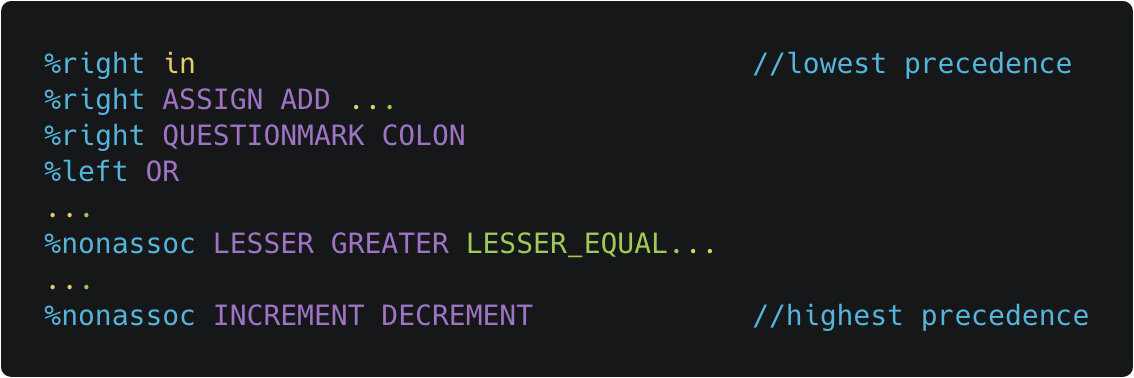
\includegraphics[width=0.7\linewidth]{images/parser/operator-precedence.png}
	\end{figure}
	\note{
		\begin{itemize}
			\item Was ist Operatoren Priorität
			\item Wie wird es in Happy implementiert
			\item Precedence top (low), bottom (high)
			\item Beschreibe Assoziativität
		\end{itemize}
	}
\end{frame}

\begin{frame}[fragile]
	\frametitle{Parser - Struktur Happy File}
	\begin{figure}[H]
		\centering
		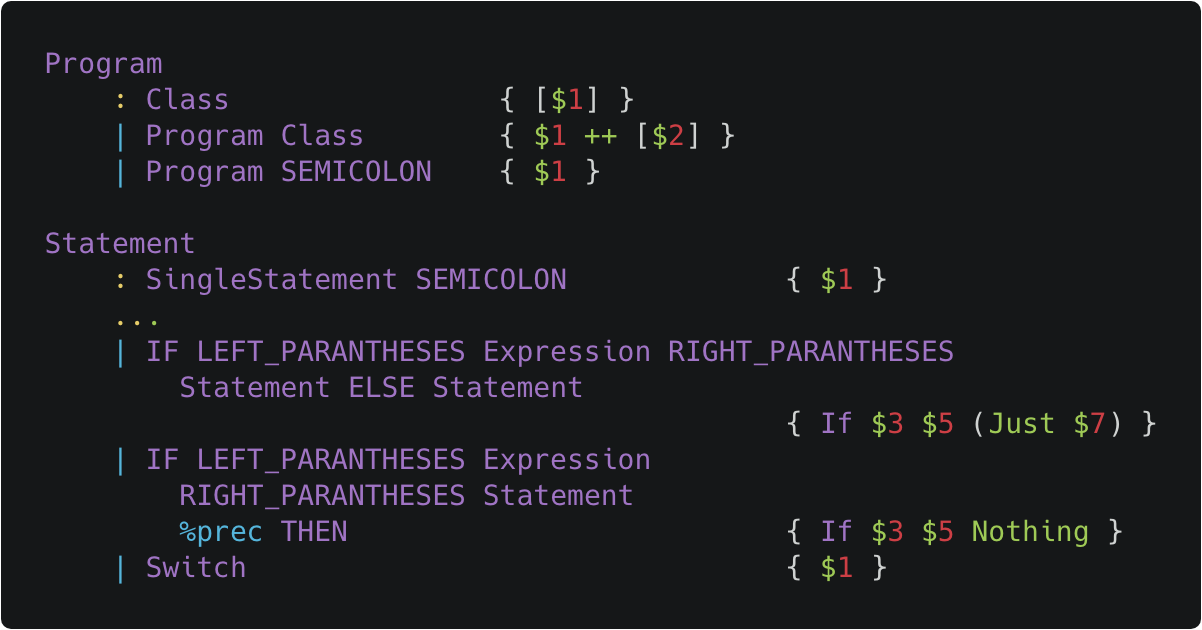
\includegraphics[width=0.7\linewidth]{images/parser/ast-example.png}
	\end{figure}
\end{frame}
\begin{frame}
	\frametitle{Parser - Klassen / Konstruktoren}
	\begin{columns}[T]
	\begin{column}{.48\textwidth}

	\begin{figure}[H]
		\centering
		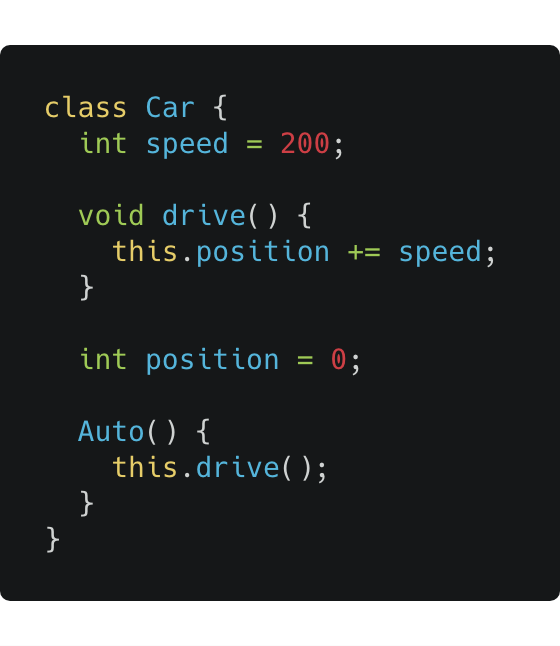
\includegraphics[width=0.6\linewidth]{images/parser/car-class.png}
		\caption{Auto Klasse}
		\label{fig:images/parser/car-class}
	\end{figure}
	\end{column}%
	\hfill%
	\begin{column}{.48\textwidth}

	\pause
	\begin{figure}[H]
		\centering
		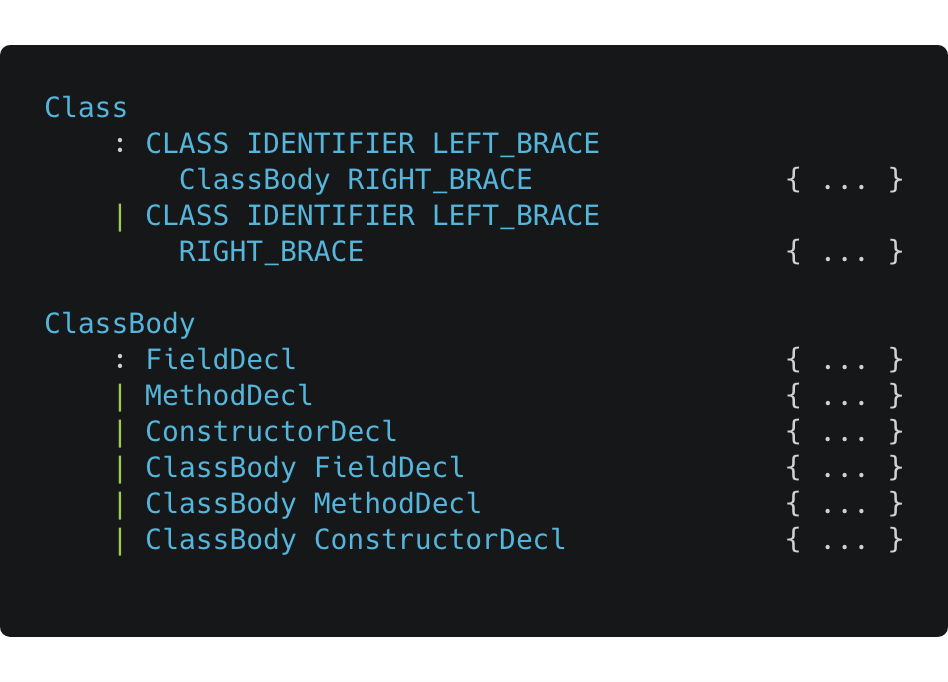
\includegraphics[width=0.95\linewidth]{images/parser/class-ast.png}
		\caption{Grammatik}
		\label{fig:images/parser/class-ast}
	\end{figure}
	\end{column}%
	\end{columns}
\end{frame}

\begin{frame}[fragile]
	\frametitle{Parser - Klassen / Konstruktoren}
	\begin{figure}[H]
		\centering
		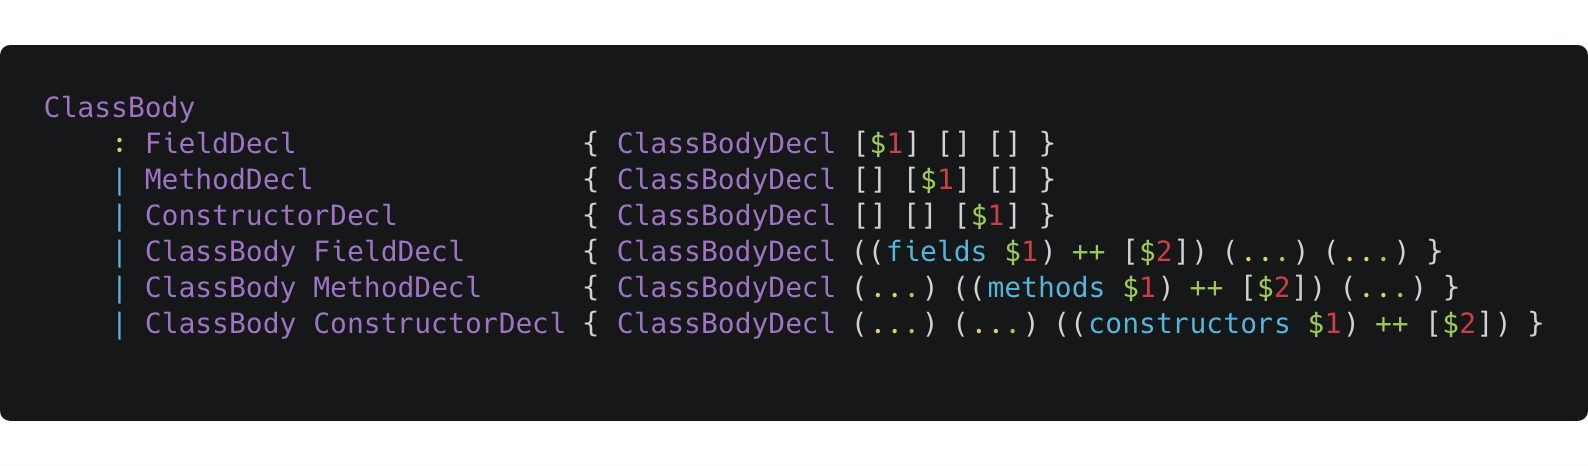
\includegraphics[width=0.9\linewidth]{images/parser/full-class-ast.png}
		\caption{Grammatik - Lösung}
		\label{fig:images/parser/full-class-ast}
	\end{figure}
\end{frame}

\begin{frame}[fragile]
	\frametitle{Parser - If - Else}
	Problem:
	\begin{figure}[H]
		\centering
		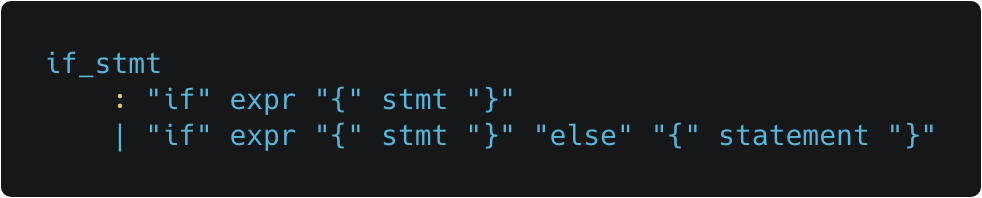
\includegraphics[width=0.7\linewidth]{images/parser/if-else-grammar.png}
	\end{figure}
	\pause
	Solution:

	\begin{figure}[H]
		\centering
		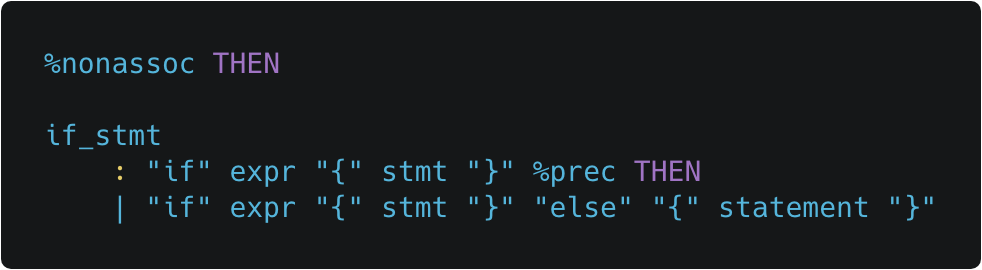
\includegraphics[width=0.7\linewidth]{images/parser/sol-if-else-grammar.png}
	\end{figure}
\end{frame}

\begin{frame}[fragile]
	\frametitle{Beispiel}
	\begin{center}
		\Huge Demo
	\end{center}
\end{frame}

